% ===== 原文 pp.43--46（tr-03 第 2 段）=====
% [原文 p.43]

\para{膜构造。} 我们知道 6d $(2,0)$ 理论 $\cX(\fsu(N))$ 是 $N$ 张重合 M5 膜的世界体理论（除去质心）。式 (4.26) 中的黎曼面可以取为一个带若干穿刺点的圆柱。于是膜构型可以描述为：$N$ 张 M5 膜缠绕在该圆柱上，并在圆柱上 $n-2$ 个点处插入横向的 M5$'$ 膜。

现在，圆周上的 M 理论就是 IIA 型弦论：缠绕圆周的 M5 膜变成 D4 膜，而位于圆周上某些点的 M5$'$ 膜变成 NS5 膜。这给出一个众所周知的膜构型 [178]：每一对相邻 NS5 膜之间都张着 $N$ 段 D4 膜：
\begin{equation}
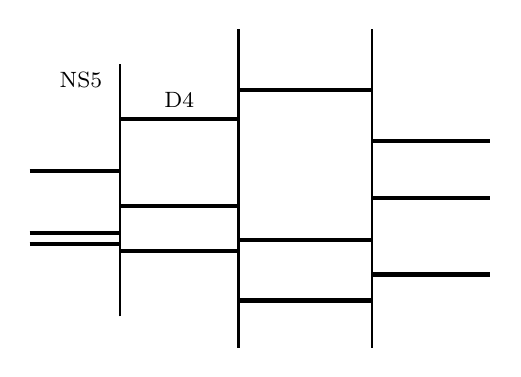
\begin{tikzpicture}[baseline=(current bounding box.center),line width=0.85pt]
  % 三条 NS5 竖线
  \draw (0,0.1) -- (0,3.3);
  \draw (1.5,-0.3) -- (1.5,3.75);
  \draw (3.2,-0.3) -- (3.2,3.75);
  % 最左侧半无限 D4
  \draw[line width=1.5pt] (-1.15,1.95) -- (0,1.95);
  \draw[line width=1.5pt] (-1.15,1.16) -- (0,1.16);
  \draw[line width=1.5pt] (-1.15,1.02) -- (0,1.02);
  % 第一、二张 NS5 之间
  \draw[line width=1.5pt] (0,2.6) -- (1.5,2.6);
  \draw[line width=1.5pt] (0,1.5) -- (1.5,1.5);
  \draw[line width=1.5pt] (0,0.93) -- (1.5,0.93);
  % 第二、三张 NS5 之间
  \draw[line width=1.5pt] (1.5,2.97) -- (3.2,2.97);
  \draw[line width=1.5pt] (1.5,1.07) -- (3.2,1.07);
  \draw[line width=1.5pt] (1.5,0.3) -- (3.2,0.3);
  % 最右侧半无限 D4
  \draw[line width=1.5pt] (3.2,2.33) -- (4.7,2.33);
  \draw[line width=1.5pt] (3.2,1.6) -- (4.7,1.6);
  \draw[line width=1.5pt] (3.2,0.63) -- (4.7,0.63);
  \node[font=\footnotesize] at (-0.5,3.1) {NS5};
  \node[font=\footnotesize] at (0.75,2.85) {D4};
\end{tikzpicture}
  \tag{4.28}
\end{equation}

这个膜图的世界体描述已知就是线性箭图规范理论 (4.26)。两个 $\mathrm{SU}(N)$ 味对称性的质量参数是两端半无限 D4 膜的位置（在图中是竖直方向的位置）。所有 $\mathrm{U}(1)$ 味对称性的质量参数，是每组 $N$ 段 D4 膜质心之间的距离。其余的竖直位置是动力学的，在规范理论一侧表现为 Coulomb 分支参数。线性箭图的 SW 曲线与微分可以从这个构型中提取出来 [178]，与 6d 视角所得一致。

在膜图中很容易容纳并不全相同的规范群秩。我们在 7.2 小节概述如何在 class S 中实现这类理论。

% [Tutor Note: p.43 式 (4.28) 与 (4.26) 的计数对应：设膜图中有 $k$ 张 NS5，则每一段夹在两相邻 NS5 之间的 $N$ 根 D4 给出一个 $\mathrm{SU}(N)$ 规范节点，共 $k-1$ 个；而 (4.26) 的规范节点数是 $n-3$，故 $k=n-2$。同理，$n$ 个穿刺点中 $0$ 与 $\infty$ 是满穿刺点，其余 $n-2$ 个是单穿刺点，对应 $n-2$ 个 $\mathrm{U}(1)$ 味节点（左端 1 个、右端 1 个、中间 $n-4$ 个）。图中 $k=3$，即 $n=5$、2 个规范节点。]

\part{第二篇\quad AGT 对应}

\section{4d 箭图的局域化}

到此为止，我们一直在 Minkowski 空间中讨论 4d $\cN=2$ class S 理论。现在转向欧氏号差。\footnote{我们将忽略 Wick 转动可能带来的困难。}本节与下一节的目标，是就 $\fg=\fsu(2)$、穿刺点为驯服的情形，解释 AGT 关系 (1.1) 的两边：
\begin{equation}
  Z_{S^4_b}\big(\mathrm{T}(\fsu(2),C,m)\big)
  =\Big\langle\widehat{V}_{\alpha_1}(z_1)\dots\widehat{V}_{\alpha_n}(z_n)\Big\rangle^{\mathrm{Liouville}}_{\overline{C}}.
  \tag{5.1}
\end{equation}

% [原文 p.44]

右边是黎曼面 $C$ 上的二维 Liouville 共形场论关联函数，它的描述推迟到第 6 节。眼下我们专注于 $\mathrm{T}(\fsu(2),C,m)$ 的球面（以及压扁球面）配分函数。5.1 小节解释如何通过耦合超引力把 4d $\cN=2$ 理论放到这一弯曲背景几何上 [179--181]（另见 [182,183] 的其他早期探索）。5.2 小节用超对称局域化，在拉氏量情形把无穷维路径积分约化为有限维的（一个矩阵模型）。所得表达式由 Nekrasov 瞬子配分函数构成，我们在 5.3 小节探讨它。超对称局域化还蕴含某些因子化性质即使对非拉氏量理论也依然成立，见 5.4 小节。

\begin{keybox}{局域化与因子化}
\begin{itemize}[leftmargin=1.4em,itemsep=1pt,topsep=1pt]
\item 4d $\cN=2$ 理论可以超对称地放在
  $S^4_b=\{y_5^2+b^2(y_1^2+y_2^2)+b^{-2}(y_3^2+y_4^2)=r^2\}\subset\R^5$ 上。
\item 对任何规范理论，超对称局域化把 $S^4_b$ 配分函数精确地化为规范群 Cartan 代数上的一个积分
  $Z_{S^4_b}=\int\dd a\,Z_{\mathrm{cl}}(a,q\bar q)\,Z_{\text{one-loop}}(a)\,Z_{\mathrm{inst}}(a,q)\,Z_{\mathrm{inst}}(a,\bar q)$。
\item 经典贡献为 $Z_{\mathrm{cl}}=|q|^{r^2|a|^2}$。
\item 单圈贡献 $Z_{\text{one-loop}}$ 只依赖于物质，对任何拉氏量理论都已知。
\item 瞬子贡献 $Z_{\mathrm{inst}}$ 关于 $q$ 全纯，对许多理论（例如线性箭图）都已知。
\end{itemize}
\end{keybox}

圆球面上的局域化在 [10] 中完成，并基于 3d 压扁球面上的一些类似进展 [184,185] 推广到压扁球面 [11]。[11] 的超引力背景在 [186] 中被推广到复的 $b$。配分函数还有另一种“Higgs 分支局域化”的表达式 [187--190]，我们用不到。关于弯曲空间局域化的综述见 [191]，专门针对 4d $\cN=2$ 理论的见 [126]。

% [Tutor Note: p.44 要点框中的 $Z_{\mathrm{cl}}=|q|^{r^2|a|^2}$ 与 p.50 式 (5.22) 的 $S_{\mathrm{cl}}=-\Re(2\pi\ii\tau)\Tr(ra)^2$ 是同一件事：由 $q=\ee^{2\pi\ii\tau}$ 得 $|q|^{r^2|a|^2}=\ee^{-\Re(2\pi\ii\tau)\,r^2|a|^2}$，而单个 Cartan 生成元上 $\Tr(ra)^2=r^2|a|^2$。这也说明 (5.22) 中半径 $r$ 的作用是让指数无量纲。]

\subsection{椭球上的理论}

\para{简单情形：圆球面。} 把 SCFT 放到圆球面 $S^4$ 上原则上是很直接的：球面是共形平坦的，只需对平直空间理论作一次共形变换。$S^4$ 上的 4d $\cN=2$ 超共形代数于是与 $\R^4$ 上的相同，即 $\fsu^*(4|2)$，其玻色部分为共形代数 $\fsu^*(4)=\fso(5,1)$ 乘以 R 对称代数 $\fu(1)$ 与 $\fsu^*(2)=\fsu(2)$。\footnote{把平直空间中的算子与球面上的算子对应起来是微妙的，因为可能存在牵涉曲率张量的混合。这一点对 4d $\cN=2$ 理论已在 [192] 中理解清楚。}

我们研究的 class S 理论（对驯服穿刺点）是 SCFT 的质量形变。因此可以把 SCFT 共形映射到球面上，再把质量作为与各味对称性耦合的矢量多重态标量的背景值打开，从而把它们放到 $S^4$ 上。结果发现质量项破坏一半超对称，把共形代数破坏为转动代数 $\fso(5)=\fsp(4)$，并把 R 对称性破坏为 $\fso(2)=\fso^*(2)$。合起来可以算出，有质量的理论保持如下超对称子代数
\begin{equation}
  \mathfrak{osp}^*(2|4)\subset\fsu^*(2|4).
  \tag{5.2}
\end{equation}

% [Tutor Note: p.44 式 (5.2) 与上一段 $\fsu^*(4|2)$ 的指标顺序不一致（原文如此）。判断依据：讨论的 4d $\cN=2$ 超共形代数标准记法是 $\fsu^*(4|2)$（4 个超荷的指标在前）；而 $\mathfrak{osp}^*(2|4)$ 把 $\fsp(4)$ 放在第二位，是子代数的标准写法。抄录时不要"统一"成同一个顺序。]

% [原文 p.45]

注意这与 $\R^4$ 上有质量理论所保持的 Poincaré 代数差别很大：例如 $\R^4$ 的空间等距群是 $\mathrm{iso}(4)=\R^4\rtimes\fso(4)$，而这里得到的是转动代数 $\fsp(4)=\fso(5)$。

AGT 对应涉及椭球（常被称为压扁球面）$S^4_b$，而不只是 $S^4$。压扁球面不是共形平坦的，在其上定义理论需要我们现在要解释的技术。

\para{共形 Killing 矢量。} 我们关心刚性弯曲空间上的量子场论（不含动力学引力）。把 Poincaré 不变的 QFT 放到弯曲空间上，做法是让理论与引力耦合、再把度规的取值冻结。\footnote{确切地说，若理论含旋量，则除度规之外还必须额外给定自旋结构（例如给定一份标架场就足够了）。}坐标变换下的不变性导致存在守恒的能量动量张量（$\nabla_\nu T^{\mu\nu}=0$）。如下一道习题所示，只要度规容许 Killing 矢量 $Y_\mu$（由 Killing 矢量方程 $\nabla_\mu Y_\nu+\nabla_\nu Y_\mu=0$ 定义），所得的弯曲空间理论就保持一部分时空（Poincaré）对称性。更一般地，若平直空间 QFT 是共形的，则 CFT 的等距与共形对称性由共形 Killing 矢量给出
\begin{equation}
  \nabla_\mu Y_\nu+\nabla_\nu Y_\mu=\frac{2}{d}\,g_{\mu\nu}\nabla_\rho Y^\rho.
  \tag{5.3}
\end{equation}

\begin{exercise}{5.1}
\begin{enumerate}[label=\arabic*.,leftmargin=2em,itemsep=1pt,topsep=1pt]
\item Poincaré 不变的定域 QFT 有一个守恒且对称的能量动量张量 $T^{\mu\nu}$。验证：若 $Y$ 是 Killing 矢量，则流 $Y_\mu T^{\mu\nu}$ 守恒。
\item 若平直空间 QFT 是共形不变的，则 $T^{\mu\nu}$ 还是无迹的。验证：此时只要 $Y$ 是共形 Killing 矢量，$Y_\mu T^{\mu\nu}$ 就守恒。提示：对方程 (5.3) 取迹，以解释其中的因子 $2/d$。
\end{enumerate}
\end{exercise}

% [Tutor Note: p.45 式 (5.3) 的因子 $2/d$ 可由取迹直接得到：设 $\nabla_\mu Y_\nu+\nabla_\nu Y_\mu=2\lambda g_{\mu\nu}$，两边用 $g^{\mu\nu}$ 缩并得 $2\nabla_\mu Y^\mu=2\lambda d$，故 $\lambda=\nabla_\rho Y^\rho/d$，代回即 (5.3)。习题 5.1 第 2 问的验证正是靠 $\lambda=\nabla_\rho Y^\rho/d$ 与 $T^\mu{}_\mu=0$ 两项相消。]

\para{共形 Killing 旋量。} 现在考虑超对称理论。这意味着存在守恒的超对称流 $G_\alpha^\mu$ 与 $\tilde{G}^{\dot\alpha\mu}$，其中 $\mu$ 是 $\mathrm{SO}(4)$ 转动群的矢量指标，$\alpha=1,2$ 与 $\dot\alpha=1,2$ 是两种手征性的旋量指标。把 $G^\mu$ 的旋量指标省略不写，守恒方程是
\begin{equation}
  D_\mu G^\mu:=\nabla_\mu G^\mu+\frac{1}{4}\omega_\mu{}^{ab}\gamma_a\gamma_b G^\mu=0,
  \tag{5.4}
\end{equation}
其中 $\nabla$ 是给定度规的 Levi--Civita 联络，$\omega$ 是其自旋联络，$a,b$ 是标架指标，$\gamma$ 是 Dirac 矩阵。

在平直空间里，要从守恒的能量动量张量得到通常的守恒平移流，做法是把 $T^{\mu\nu}$ 与一个常平移矢量 $a_\mu$ 缩并。这里类似：对常旋量 $\xi$ 有通常的流 $\xi G^\mu=\xi^\alpha G_\alpha^\mu$ 与 $\tilde{\xi}\tilde{G}^\mu=\tilde{\xi}_{\dot\alpha}\tilde{G}^{\dot\alpha\mu}$。\footnote{这里我们使用了一个常见的措辞滥用：谈论常旋量需要选定一份标架场，我们取平直空间上标准的笛卡儿标架。}在弯曲空间中可以验证：只要 $\xi$ 是 Killing 旋量，$\xi G^\mu$ 就守恒：
\begin{equation}
  D_\mu\xi:=\left(\partial_\mu+\frac{1}{4}\omega^{ab}_{\ \ \mu}\gamma_a\gamma_b\right)\xi=0.
  \tag{5.5}
\end{equation}

% [原文 p.46]

（注意我们写 $\partial$ 而不写 $\nabla$，因为 $\xi$ 没有矢量指标。）

正如 $x_\mu T^{\mu\nu}$ 守恒意味着理论共形不变，$x^\nu\gamma_\nu G^\mu$ 按 (5.4) 的意义守恒则意味着理论超共形不变。放到弯曲空间上后，只要时空容许共形 Killing 旋量，理论就具有超（共形）对称性：
\begin{equation}
  D_\mu\xi=\frac{1}{d}\gamma_\mu\gamma^\nu D_\nu\xi.
  \tag{5.6}
\end{equation}

\begin{exercise}{5.2}
验证：若理论是超共形的，(5.6) 确实给出守恒流 $\xi G$。
\end{exercise}

\para{广义 Killing 旋量。} 我们在 3.1 小节把（部分）拓扑扭曲定义为某些转动与 R 对称性的混合，这使我们能把 6d $(2,0)$ 理论紧化在黎曼面 $C$ 上。只要平直空间理论具有 R 对称性流 $J^\mu$，这个想法就可以如下细化并推广。把 QFT 放到弯曲空间上时，除了与 $T^{\mu\nu}$ 耦合的度规 $g_{\mu\nu}$ 之外，我们还可以打开一个与 $J^\mu$ 耦合的背景规范场 $V_\mu$（我们通常不打开与超对称流耦合的费米子背景）。

在这样的背景中，Killing 旋量方程 (5.5) 通过把 R 对称性规范场纳入协变导数而得到推广：
\begin{equation}
  D_\mu\xi:=\left(\partial_\mu+\frac{1}{4}\omega^{ab}_{\ \ \mu}\gamma_a\gamma_b+V_\mu\right)\xi=0.
  \tag{5.7}
\end{equation}
共形 Killing 旋量方程也以同样的方式、用新的 $D_\mu$ 推广到 (5.6)。这里 $V_\mu\xi$ 应按给定 R 对称性下的 R 荷作相应的权重，这是有规范场时协变导数的标准做法。（部分）拓扑扭曲就是选择 $V_\mu$ 去抵消 $\omega^{ab}_{\ \ \mu}$ 的某个分量，使 $\xi$ 的相应分量可以直接取为（沿 $C$ 的）常数。更一般的背景规范场 $V$ 选取，可以使我们即使所关心的弯曲流形没有任何（共形）Killing 旋量，也能保持一部分超对称性。

\para{压扁球面。} [11] 中为把 4d $\cN=2$ 理论放到 $S^4_b$ 上而找到的超引力背景相当复杂，它把超引力多重态中大多数玻色场都取为非零值。具体表达式请参见综述 [126]。对我们而言只需其中两个方面。度规是由欧氏 $\R^5$ 的度规在如下嵌入下诱导的
\begin{equation}
  S^4_b:=\{y_5^2+b^2(y_1^2+y_2^2)+b^{-2}(y_3^2+y_4^2)=r^2\}\subset\R^5.
  \tag{5.8}
\end{equation}
4d $\cN=2$ 超对称的一部分得以保留：$y_1,y_2$ 平面与 $y_3,y_4$ 平面内的 $\mathrm{U}(1)^2$ 转动 $M_{12}$ 与 $M_{34}$，以及一个超荷 $Q$（及其共轭），满足
\begin{equation}
  Q^2=\frac{b}{r}\big(M_{12}-\tfrac{1}{2}J_3^{\mathrm{R}}\big)
     +\frac{1}{br}\big(M_{34}-\tfrac{1}{2}J_3^{\mathrm{R}}\big),
  \tag{5.9}
\end{equation}
其中 $J_3^{\mathrm{R}}$ 是 $\fsu(2)_{\mathrm{R}}$ 的 Cartan 生成元。

% [Tutor Note: p.46 式 (5.9) 两项都带 $-\frac{1}{2}J_3^{\mathrm{R}}$（原文如此，不是抄录错误）。核对思路：取 $b=1$ 时 $Q^2=\frac1r(M_{12}+M_{34}-J_3^{\mathrm{R}})$，应与 [10] 中圆球面的超荷平方相符；$b\ne1$ 时两平面系数分别为 $b/r$ 与 $1/(br)$，这一不对称正是"压扁"的体现。若在别处见到两项符号相反，多半是把 $M_{34}$ 所在平面的定向取了反。]
